
%(BEGIN_QUESTION)
% Copyright 2006, Tony R. Kuphaldt, released under the Creative Commons Attribution License (v 1.0)
% This means you may do almost anything with this work of mine, so long as you give me proper credit

The issue of {\it inherent characteristic} versus {\it installed characteristic} for process control valves has an interesting parallel in the world of semiconductor electronics: the behavior of transistors under ideal (constant supply voltage) versus realistic (loaded) conditions:

$$\includegraphics[width=15.5cm]{i01387x01.eps}$$

In order to understand how the ideal behavior of a transistor maps to the real (``installed'') world of an amplifier circuit, we can sketch something called a {\it load line} on the same graph where we draw the transistor's characteristic curves.

Explain what a ``load line'' is and what it means for a transistor circuit.

\underbar{file i01387}
%(END_QUESTION)





%(BEGIN_ANSWER)

A ``load line'' describes how much voltage is available to power a transistor for any given amount of collector current:
 
$$\includegraphics[width=15.5cm]{i01387x02.eps}$$

\vskip 10pt

Note: the amount of load resistance suggested by the load line in the above graph is 2.67 k$\Omega$.

%(END_ANSWER)





%(BEGIN_NOTES)


%INDEX% Electronics review: load lines
%INDEX% Final Control Elements, valve: characterization

%(END_NOTES)


